\lhead{\emph{Study on Parameter Tuning}}

\chapter{Study on Parameter Tuning}
In this section, we will perform in depth analysis on different parameters and the trade off between the two algorithm (Histogram and Partially Sorted). Different parameters will yield different result and base on the different dataset. The experiment method will be the same as the evaluation section where we will be using the same dataset. However, we will only limits to real-world dataset and one of the distribution due to the computation power in testing all of the distribution. We expect that the result will help gain more understanding on different parameters that the histogram and partially sorted introduced and its flaws and tradeoff.

\section{Histogram Bin} \label{Histogram Bin}
\begin{figure}[H]
    \centering
    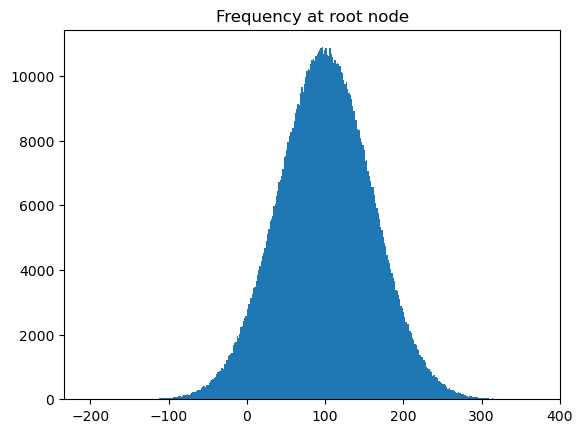
\includegraphics[width=100mm,scale=1]{Figures/GaussianDistributionRootNode.png}
    \caption{
     Distribution at root node
    }
    \label{fig:DistRootNode}
\end{figure}
The choice of the bin size is important consideration when maintaining a histogram in each node. The bin size determines the number of bins used in the histogram and the range of values includes in each bin. The bin size should be chosen carefully to ensure that the resulting histogram accurately reflects the distribution of the data. 

If the bin size is too small, the histogram may not be able to capture the distribution of keys in the node and difficult to interpret. This is because each bin will contain only a small number of data points, and the resulting bar heights will be highly variable. Which makes it difficult to see the underlying pattern of the data.  

On the other hand, if the bin size is too large, the resulting of the histogram in each node may be too coarse and may not accurately capture the fine details of the distribution. This will result in important details to be missed out. 

We tested small static bin and the \acrshort{fdrule} to gain some insights on the data patterns and how bins affect the gaps optimization. The figure \ref{fig:DistRootNode} is taken from the histogram \acrshort{lipp} root node with a Gaussian distribution dataset on one million keys. we can see that the root node will contain the whole tree distribution. 

In this section, we will test the static bin size and Freedman-Diaconis rule to find the appropriate bin size and its tradeoff using the same dataset and setup as the previous section. However, in our calculation of the $bin\_index$, we have to find the $bin\_width$ which determines the range of keys that fall into this index. For example, if $bin\_width$ is equal to $1$,  that means the range of first index can be in the range of keys $0$ to $1$. With static bin size, we can calculate $bin\_width$ by $\frac{Key_{max} - Key_{min}}{bin\_size}$.

\subsection{Gaussian Distribution} 
\begin{figure}[H]
    \centering
    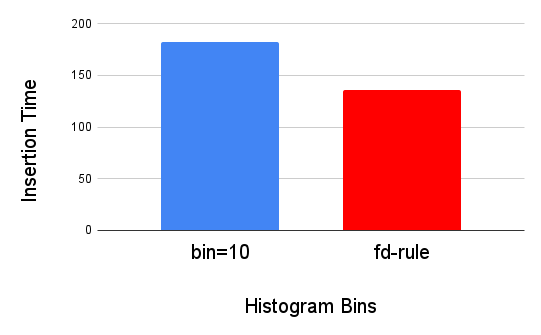
\includegraphics[width=100mm,scale=1]{Figures/InsertionHistBin.png}
    \caption{
     Results of Insertion on Different Histogram Bin Setting
    }
    \label{fig:InsertionHistBin}
\end{figure}
\begin{figure}[H]
    \centering
    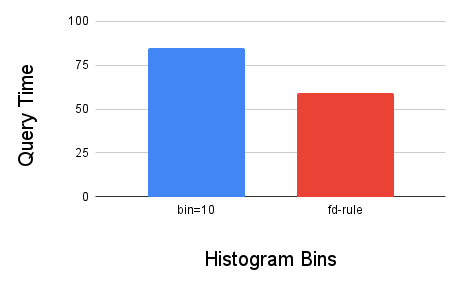
\includegraphics[width=100mm,scale=1]{Figures/QueryHistBin.png}
    \caption{
     Results of Query on Different Histogram Bin Setting
    }
    \label{fig:QueryHistBin}
\end{figure}
In this section, we aim to compare the performance of a static bin size of $10$ with the \acrshort{fdrule} when used in the histogram-based \learnindex algorithm on Gaussian Distribution. We carried out the same tests as in the previous section, but with the addition of comparing the performance of the different bin sizes.

From the resulting figure \ref{fig:InsertionHistBin} and \ref{fig:QueryHistBin}, we can observe that using a static bin size of $10$ does not perform well when there is a large amount of data in the tree. This is because the root node, which represents the entire distribution of the tree, does not capture the pattern well when the bin size is too small. As a result, the gap optimization in the tree performs poorly, causing the tree to grow deeper and impacting the read and write operations since they are bounded by $O(h)$ where $h$ is the height of the tree. Furthermore, we can also see that both the insertion and query operations perform poorly due to the increasing height of the tree when the gap optimization does not work well. Additionally, the number of \conflict (or new nodes created) also increases, as the histogram-based \learnindex relies heavily on the histogram in each node to distribute gaps according to the frequencies.
\begin{figure}[H]
    \centering
    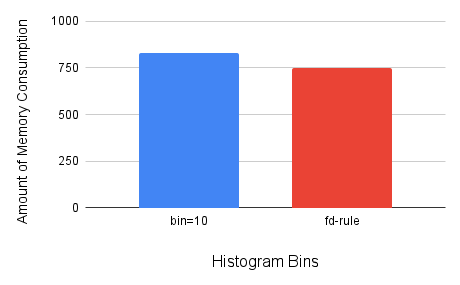
\includegraphics[width=100mm,scale=1]{Figures/MemoryHistBin.png}
    \caption{
     Results of Memory Consumption on different histogram bin setting
    }
    \label{fig:MemoryHistBin}
\end{figure}
In contrast, the \acrshort{fdrule} maintains a longer frequency (or bin) size, which consumes more memory compared to the static bin size. From the resulting figure \ref{fig:MemoryHistBin}, we can see that the \acrshort{fdrule} maintains larger number of bin sizes, while the static bin size only maintains $10$. This cost will be incurred when the adjustment triggers, and the algorithm has to rebuild the nodes. However, it offsets the operation cost, as the insertion operation has to traverse less depth compared to the static bin size. 

This makes the \acrshort{fdrule} performs well in term of representing the underlying patterns and able to make our gaps optimization works well on different distributions. It outperforms the static bin size when perform operations like the insertion, query and deletion due to the smaller depth that it has to traverse down.


\subsection{Real-World Dataset (Longitudes)} 
\begin{figure}[H]
    \centering
    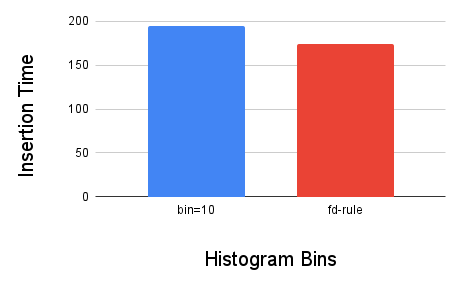
\includegraphics[width=100mm,scale=1]{Figures/InsertionHistBinLogi.png}
    \caption{
     Results of Insertion Operation on different histogram bin setting
    }
    \label{fig:InsertionResultLogi}
\end{figure}
Real-world datasets can have a complex distribution, and unlike synthetic datasets with known distributions, it can be challenging to predict the distribution of new keys. Therefore, it is important to evaluate the performance of the \learnindex algorithms on real-world datasets to understand how they adapt to the underlying patterns.

Based on the results of our experiments on real-world datasets, we observed that the performance of the histogram \learnindex was poor compared to the baseline, as discussed in the previous section. However, in this experiment, we evaluated the performance of two different approaches, namely the static bin size and the \acrshort{fdrule}.

The results showed that both the static bin size and the \acrshort{fdrule} did not perform well when the distribution of new keys was unknown, as they were not able to capture the underlying patterns of the dataset. As a result, both approaches performed poorly on insertion and query operations compared to the baseline. However, the \acrshort{fdrule} still outperforms the static bin size as it is able to capture keys' distribution better than the static bin size which overfits to only a few scenarios (Figure \ref{fig:InsertionResultLogi}).

\begin{figure}[H]
    \centering
    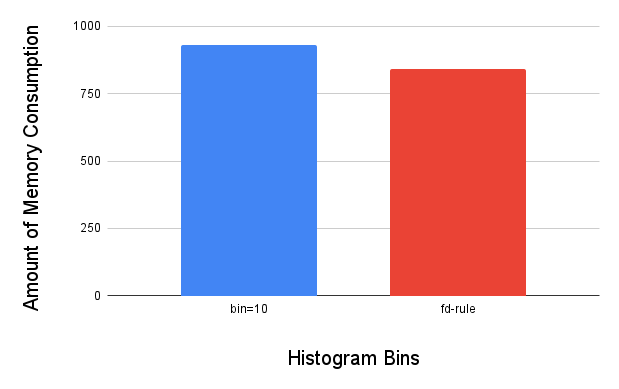
\includegraphics[width=100mm,scale=1]{Figures/MemoryHistBinLogi.png}
    \caption{
     Results of Memory Consumption on different histogram bin setting
    }
    \label{fig:MemoryConsumptionLogi}
\end{figure}

For memory consumption (Figure \ref{fig:MemoryConsumptionLogi}), the \acrshort{fdrule} still performs better than the static bin size. The \acrshort{fdrule} is able to capture the distribution better than the static bin size. Static bin size may only work in a few scenarios where there is not large amount of data. In this case, it makes static bin size create more child nodes than the \acrshort{fdrule} which consumes more memory to maintain the child nodes.

Therefore, based on our experiments on one million real-world keys, the \acrshort{fdrule} approach is a better solution for both real-world dataset and static dataset. This is because the \acrshort{fdrule} is able to capture distribution and distribute gaps based on the detailed distribution while the static bin size will only works if there is lesser data and require a lot of engineering efforts to tune this parameter to work on different scenarios. 



\section{Partially Sorted $\epsilon$ Spaces}
The $\epsilon$ spaces are a crucial factor in determining the performance of \learnindex, as it influences the traversal of the tree and the operation's runtime complexity. The $\epsilon$ parameter determines the number of gaps to search for in the gapped array when the predicted position is not empty. As all the operations are bounded by the $\epsilon$ spaces, the number of $\epsilon$ sets affects the search performance.

To determine the impact of the $\epsilon$ parameter on the search operation, we conducted experiments on different parameter values, namely $1$, $5$, and $10$, using the same datasets as in the previous section, i.e., Gaussian and Real-World datasets. We evaluated the performance of the insertion, query, and deletion operations using these different parameter values.

The $\epsilon$ parameter has a significant impact on the search operation's performance. In general, a larger value of $\epsilon$ will result in a higher number of gaps to search for, making the search operation more efficient as query has to traverse down lesser depth due to smaller tree heigit. However, a larger value of $\epsilon$ also increases the memory overhead of the index, as more gaps need to be stored. 

On the other hand, a smaller value of $\epsilon$ will result in fewer gaps to search for, making the new node creation higher which will make the search operation in efficient. However, a smaller value of $\epsilon$ also reduces the number of search after the non-empty spaces.


\subsection{Gaussian Distribution}
\begin{figure}[H]
    \centering
    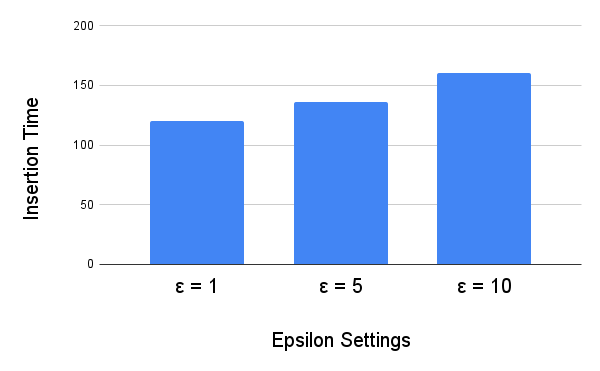
\includegraphics[width=100mm,scale=1]{Figures/InsertionGauEp.png}
    \caption{
     Results of Insertion Operation on different Partially Sorted $\epsilon$ spaces
    }
    \label{fig:InsertionGauEp}
\end{figure}
\begin{figure}[H]
    \centering
    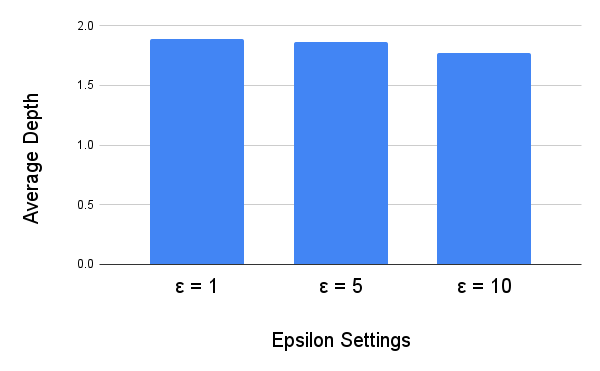
\includegraphics[width=100mm,scale=1]{Figures/AvgTreeEpGau.png}
    \caption{
     Results of Average Tree Depth on different Partially Sorted $\epsilon$ spaces
    }
    \label{fig:AverageTreeDepthGauEp}
\end{figure}
In the case of the Gaussian Distribution, we inserted keys with the same distribution as the keys that were already present in the tree. However, we do not expect the partially sorted data structure to perform well on this distribution as it only delays the slow operation of new node creation until the gaps are full. The results from the Insertion operation Figure \ref{fig:InsertionGauEp} shows that the trend of results changes as the number of $\epsilon$ decreases, indicating that the insertion operation becomes faster as the number of searches it has to perform decreases. However, if we look at the Figure \ref{fig:AverageTreeDepthGauEp}, we can see that the number of new node creations increases as the number of $\epsilon$ decreases. This is because it has lesser $\epsilon$ spaces for the partially sorted to delay new node creation. 

In addition, querying keys in the partially sorted data structure has the same performance trend as the insertion operation. This is because they both have the same time complexity, which is $O(\epsilon+\log N)$. This complexity is bounded by the search after the predicted position. Based on our results, it seems that the time to search a key is mostly dominated by the $\epsilon$ linear search as the trend of the search performance seem to decreases while the $\epsilon$ also decreases. However the number of nodes creation inversely related to the $\epsilon$ because the smaller the $\epsilon$, the number of lesser gaps to delay new node creation. 

The importance of the $\epsilon$ parameter in the partially sorted data structure is enormous, as all operations are mostly bounded by the traversals down the tree height and the $\epsilon$ spaces (or $O(\epsilon+\log N)$). The $\epsilon$ parameter determines the number of gaps in the gapped array to search for when the predicted position is not empty. Since all operations are bounded by the $\epsilon$ spaces, the number of $\epsilon$ sets will affect the search performance. 

Furthermore, its effectiveness heavily depends on the choice of the parameter $\epsilon$, which determines the number of gaps to search for when the predicted position of a key is not empty. This choice can require significant engineering effort, and even with a well-chosen $\epsilon$, partially sorted may not outperform other data structures.

In comparison to baseline and histogram data structures, which are only bounded by the height of the tree, partially sorted suffers from the need to delay the creation of new nodes until gaps are filled. This means that partially sorted does not assume any underlying pattern in the data distribution, but instead aims to optimize search and insertion by using the gaps as a buffer.

\subsection{Real-World Dataset (Longitudes)} 
\begin{figure}[H]
    \centering
    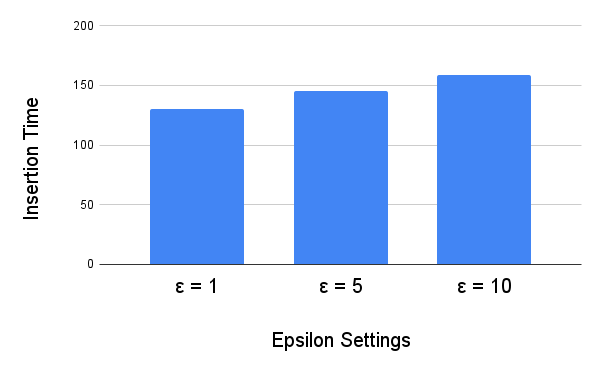
\includegraphics[width=100mm,scale=1]{Figures/InsertionLogEp.png}
    \caption{
     Results of Insertion Operation on Different Partially Sorted $\epsilon$ Spaces 
    }
    \label{fig:InsertionLogEp}
\end{figure}
\begin{figure}[H]
    \centering
    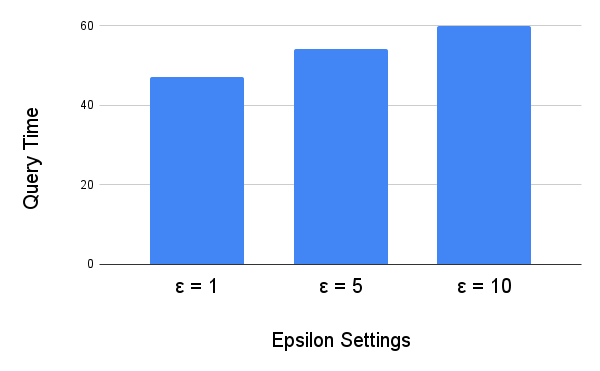
\includegraphics[width=100mm,scale=1]{Figures/QueryLogEp.png}
    \caption{
     Results of Query Operation on Different Partially Sorted $\epsilon$ Spaces 
    }
    \label{fig:QueryLogEp}
\end{figure}
When applied to real-world datasets, the partially sorted algorithm demonstrates a similar performance trend to that seen in static scenarios. When compared to other algorithms such as baseline and histogram, the partially sorted algorithm may not always be the most efficient. Nevertheless, this section of our study focuses on comparing the performance of different partially sorted parameter settings.

The results presented in the figure \ref{fig:InsertionLogEp} and \ref{fig:QueryLogEp} clearly show that partially sorted with $\epsilon = 1$ performs best in operations such as insertion, deletion, and query. This is because this setting only requires one space search after the predicted position, which can significantly improve the algorithm's performance. Since the time complexity of the algorithm is bounded by $\epsilon+\log N$, a lower value of $\epsilon$ leads to faster operations.
\begin{figure}[H]
    \centering
    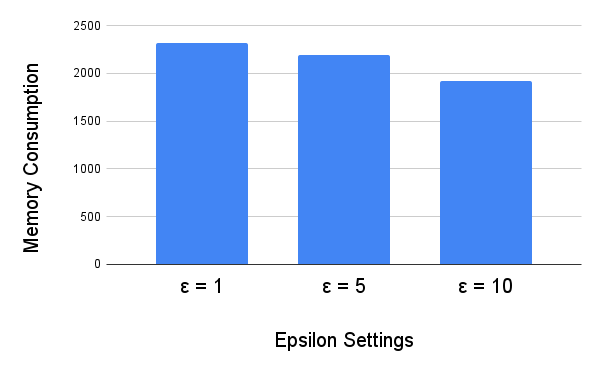
\includegraphics[width=100mm,scale=1]{Figures/MemoryLogEp.png}
    \caption{
     Results of Memory Consumption on Different Partially Sorted $\epsilon$ Spaces 
    }
    \label{fig:MemoryLogEp}
\end{figure}
However, when $\epsilon$ is decreased, the memory consumption of the algorithm increases (Figure \ref{fig:MemoryLogEp}). This is in line with our expectations, as reducing the number of spaces only delays the new node creation process for one conflict. As a result, there are more child nodes with lower $\epsilon$ values, leading to increased memory usage.

In summary, the value of $\epsilon$ in partially sorted refers to the number of limits that the algorithm can locate, which only delays the new node creation process. This algorithm does not take advantage of the underlying pattern of the keys, making its results similar for both real-world datasets and static scenarios. Therefore, selecting the optimal value of $\epsilon$ for a given dataset is critical to achieving the best performance of the partially sorted algorithm.

\section{Tradeoff}
Tradeoff is a crucial aspect of designing a \learnindex structure as it involves balancing size, accuracy, and efficiency. However, the accuracy can be eliminated by introducing new node creation in \acrshort{lipp} algorithm \cite{LIPP}, which leads to exact predictions but increases the size of the structure as a new node is created each time the predicted location is already occupied. In contrast, the partially sorted algorithm introduces the accuracy tradeoff in terms of $\epsilon$ which determines the number of keys that can be located in the structure.

In this section, we will compare the tradeoffs between Histogram and Partially Sorted parameters using the results obtained in the previous section. Although the Histogram algorithm does not require an accuracy tradeoff as the predicted position is exact and the time complexity is bounded by the height of the tree. In contrast, Partially Sorted provides a balance between accuracy, size and efficiency tradeoffs, but it may not perform as efficiently as Histogram or other algorithms in certain scenarios. Therefore, it is important to consider the specific use case and requirements when deciding which algorithm to use.

\subsection{Histogram}
In the previous section on \nameref{Histogram Bin}, we compared the performance of different bin sizes in a static scenario with a Gaussian Distribution. We found that the histogram outperformed the baseline and partially sorted algorithms. However, we also found that the choice of bin size plays a significant role in the accuracy and efficiency of the algorithm. If the bin size is too small, the histogram will not be able to capture the distribution of keys in the tree, resulting in poor accuracy. On the other hand, if the bin size is too large, the distribution will be too coarse, also resulting in poor accuracy. Hence, there is a tradeoff between bin size and the visibility of underlying patterns.

In terms of memory consumption, a \acrshort{fdrule} is the best option. However, this approach sacrifices the node size as it has to maintain higher size of frequencies array. Furthermore, the static bin size require fine tuning which consequently lead to more conflicts, and the \learnindex will have to create more new nodes, making operations less efficient. Tuning for a good enough bin size becomes challenging as the tree grows larger, and each node has its own distribution, which cannot use a "one size fits all" approach. However, if we compare with the baseline, the histogram algorithm consumes more memory as it has to maintain the frequency array to distribute gaps while baseline does not have extra array in each node.

In addition, \acrshort{fdrule} helps determine the bin size based on the keys in each node. This approach decides the bin size in each node such that it is good enough to distribute gaps based on the frequencies array. However, the tradeoff for this implementation is that it will consume more memory in each node as it has to maintain the array of frequencies. Due to variable bin size, the accuracy of distributing gaps increases, which decreases the number of conflicts. Thus, operations performance increases, as seen from the previous section.

From our experiment, we conclude that using \acrshort{fdrule} is the best approach as it determines a good enough bin size for each node, resulting in higher accuracy and fewer conflicts. However, controlling the amount of memory consumption can be challenging. It is essential to balance memory consumption and performance to achieve the optimal solution. We argue that optimizing operations performance is the best approach since insertion and query operations occur frequently in real-world systems where users have to keep the data updated. Thus, the efficiency of these operations plays a critical role in the overall system performance.


\subsection{Partially Sorted} 
In this section, we discuss the tradeoff between size, efficiency and accuracy in the context of \learnindex with partially sorted arrays. Unlike histogram bins, partially sorted arrays use the concept of partial limit spaces or $\epsilon$ to delay the slow new node creation by storing it a few $\epsilon$ spaces after predicted position. $\epsilon$ defines the number of spaces that the algorithm has to search for after the predicted position. Therefore, the operation performance like insertion is bounded by $\epsilon + \log N$, where $N$ is the number of keys in the node. In this section, we will be experimenting with different values of $\epsilon$ to determine the tradeoff between size, efficiency, and accuracy.

From the experimental results in Figure \ref{fig:InsertionGauEp}, we observe that the operation performance of partially sorted arrays decreases as $\epsilon$ increases. This is consistent with the theoretical analysis that suggests that the performance is not only bounded by $\log N$, but also by the $\epsilon$ spaces that the algorithm has to search. On the other hand, partially sorted arrays do not need to store any extra information like histogram bins, where a frequency array is maintained for each node. To determine if a key is partially sorted or not, we simply use the model to predict the position of the key and compare it with the current position. If the predicted position is different from the current position, then it is a partially sorted key.

In terms of operation performance, we observe that insertion is the most impacted operation by the choice of $\epsilon$. The reason for this is the recursive rebuild operation that is triggered when the $\epsilon$ spaces are exhausted. In particular, when the number of partially sorted keys in the node is high, the number of recursive rebuild operations required also increases, thereby reducing the efficiency of the insertion operation.

Based on the experimental results, we can conclude that $\epsilon = 1$ offers the best tradeoff between size and performance in terms of operations like insertion. However, as $\epsilon$ increases, the performance of the partially sorted array also improves, but at the cost of increased memory consumption due to the need to store more partially sorted keys. For example, when $\epsilon = 5$, the performance of insertion is significantly worse than when $\epsilon = 1$ due to the increased number of recursive rebuild operations required to insert a new key.

In conclusion, the choice of $\epsilon$ in partially sorted arrays determines the tradeoff between size, efficiency, and accuracy. While a smaller value of $\epsilon$ improves the performance of operations like insertion, a larger value of $\epsilon$ improves the memory consumption of the algorithm at the cost of increases in operation time. Therefore, it is important to strike a balance between these tradeoffs when implementing \learnindex with partially sorted arrays.



\section{Maximum Gaps}
In this section, we will delve deeper into an experiment to explore how different gaps distributions affect the performance and memory consumption of Histograms. This experiment is essential because the number of gaps that we distribute will affect the overall usage of memory as the gaps have to be reserved for key insertion.

In this experiment, we will test different datasets, such as Gaussian distributions and real-world datasets, to observe the changing trends and the trade-offs on different settings of gap distribution. We will also test different gap distributions such as $2\times$, $2.5\times$, and $3\times$. The $2\times$ refers to double the size of keys currently collected in the adjustments. The adjustment or branch pruning is only done based on the mentioned condition. For example, if we collected keys of $[1,2,3]$, the size of the expanded array will be $2\times 3$ which is $6$ so there will be $3$ keys and $3$ gaps. However, for $2.5\times$ the size, if the outcome of multiplication contains a decimal, we will round it up and place the leftover gaps at the end of the array.

\begin{figure}[H]
    \centering
    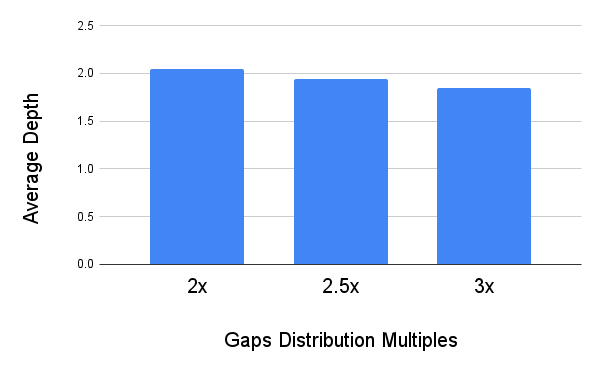
\includegraphics[width=100mm,scale=1]{Figures/AVGGauMaxGaps.png}
    \caption{
     Results of Average Tree Height on Different Maximum Gaps Parameters (Gaussian Distribution)
    }
    \label{fig:AvgMaxGapsGau}
\end{figure}
In the experiment on the Gaussian distribution, the results in figure \ref{fig:AvgMaxGapsGau} show that distributing gaps $3\times$ the size of keys collected performs best in terms of new node creation, as it has more gaps to locate keys in, which will reduce the number of child nodes. This setting can also increase the operation performance like insertion, as it traverses to a lesser depth than the $2\times$ and $2.5\times$ settings.
\begin{figure}[H]
    \centering
    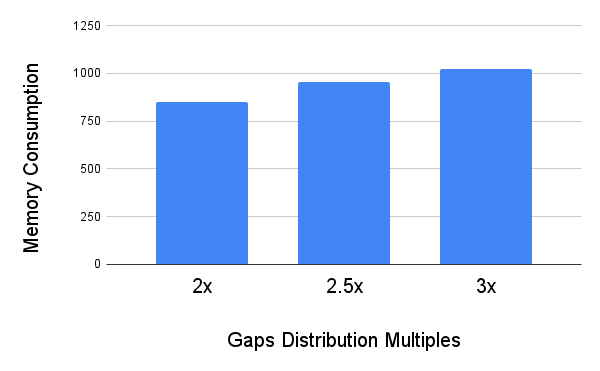
\includegraphics[width=100mm,scale=1]{Figures/MemoryMaxGapsGau.png}
    \caption{
     Results of Memory Consumption on Different Maximum Gaps Parameters (Gaussian Distribution)
    }
    \label{fig:MemoryMaxGapsGau}
\end{figure}
However, the memory consumption is affected by the increasing number of gaps, which is a tradeoff between size and efficiency. From the memory consumption figure \ref{fig:MemoryMaxGapsGau}, we can see that the amount of memory consumed by $3\times$ increases from $2\times$ and $2.5\times$. Even though $3\times$ has lesser tree depth, but reserving more gaps in each nodes consumes more memory than the amount of new child nodes created by $2\times$.

If the operation performance is the main concern, distributing more gaps can help reduce the number of new node creations while consuming more memory, as the gaps must be reserved for new keys, which is in line with the theoretical analysis that the performance is bounded by the height of the tree ($O(\log N)$). That means if we can reduce the height of the tree, we will gain performance in operations like insertion, deletion, and query. However, if memory is the primary concern, distributing more gaps will consume more memory.

From our testing, it seems that the $2\times$ setting is the best tradeoff between operation performance and memory consumption, as the average tree height trend does not increase as much as the memory consumption. From the figure \ref{fig:MemoryMaxGapsGau}, we can see that the $3\times$ gaps distribution increases memory consumption much more than it increases operation performance. Which makes $2\times$ the best tradeoff in performance and size. 
\begin{figure}[H]
    \centering
    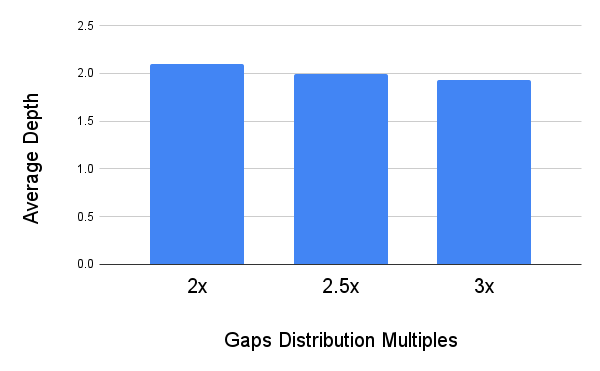
\includegraphics[width=100mm,scale=1]{Figures/AvgLogMaxGaps.png}
    \caption{
     Results of Average Tree Height on different Maximum Gaps Parameters (Longitudes Distribution)
    }
    \label{fig:AvgLogMaxGaps}
\end{figure}
For the real-world dataset, a similar trend appears that the maximum number of gaps to distribute will have more gaps for the model to insert new keys into. Based on the figure \ref{fig:AvgLogMaxGaps}, we can see that the $3\times$ performs better in terms of average tree height as it reduces the number of new child nodes because it has more gaps for the machine learn index to place new keys in. When there are fewer child nodes, the operation performance increases, which is in line with the theoretical analysis, where the operation performance for histograms is bounded by how much the height of the tree grows.
\begin{figure}[H]
    \centering
    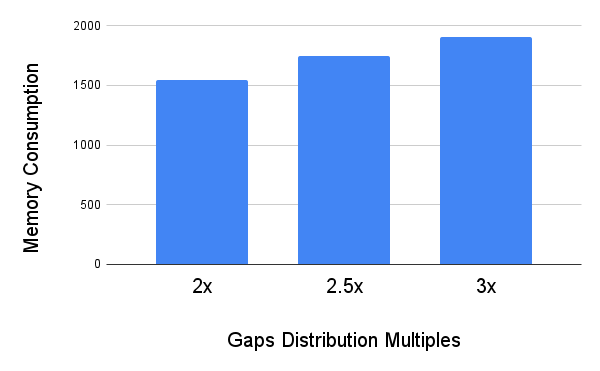
\includegraphics[width=100mm,scale=1]{Figures/MemoryLogMaxGaps.png}
    \caption{
     Results of Memory Consumption on different Maximum Gaps Parameters (Longitudes Distribution)
    }
    \label{fig:MemoryLogMaxGaps}
\end{figure}
However, expanding more gaps $3\times$ consumes extra memory (figure \ref{fig:MemoryLogMaxGaps}) as the gaps have to be reserved for new keys, which will consume memory. Furthermore, we can see from the figure \ref{fig:MemoryLogMaxGaps} that the amount of memory consumption increases when we distribute more gaps. However, the gain in operation performance is not significant and does not outweigh the fact that memory consumption trend increases higher than the operation performance. Which makes $2\times$ the number of collected keys the best tradeoff between operation performance and memory consumption in real-world datasets.

In conclusion, distributing more gaps can help reduce the number of new node creations and increase operation performance, but at the expense of memory consumption. The optimal gap distribution is a tradeoff between operation performance and memory consumption, with $2\times$ being the best setting for most scenarios.

\section{Scalability}

In this section, we will delve into the scalability of two indexing algorithms, namely the histogram and partially sorted index, by analyzing their performance on datasets of varying sizes. We will be using the same datasets as the previous section, but this time with an increase in the number of insertions. We will test on datasets with sizes of $10M$, $20M$, and $50M$ and also perform tests on both Gaussian distribution and real-world datasets.

The performance of an indexing algorithm is crucial when dealing with large datasets as it determines the speed of insertion, query, and building. A good indexing algorithm should be able to handle large datasets efficiently, without sacrificing performance. The scalability of an indexing algorithm is, therefore, an important factor to consider when selecting an indexing algorithm.

To test the scalability of the histogram and partially sorted index, we will perform insertion, query, and building operations on datasets of varying sizes. We will start by inserting $10M$ keys into both indexing algorithms and measure their performance. We will then repeat the process with datasets of sizes $20M$ and $50M$.

Additionally, we will test the scalability of the algorithms on two different types of datasets. The first type is the Gaussian distribution, which is a well-known distribution often used to test algorithms. The second type is a real-world dataset, which is more complex and closer to the kind of data an algorithm would encounter in a practical scenario.
\begin{figure}[H]
    \centering
    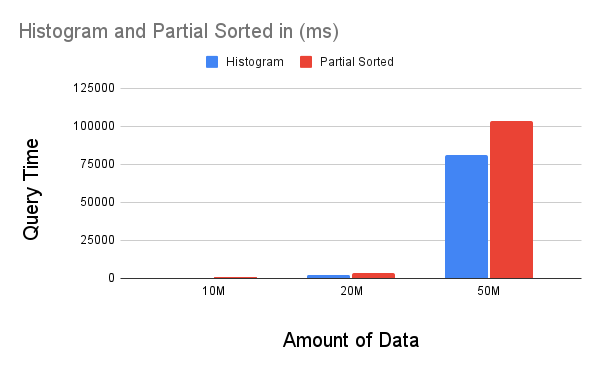
\includegraphics[width=100mm,scale=1]{Figures/QueryScalability.png}
    \caption{
     Results of Query Operation on different test sizes (Gaussian Distribution)
    }
    \label{fig:QueryScalability}
\end{figure}
When it comes to query performance on Gaussian Distribution, the histogram has a clear advantage over the partially sorted approach (Figure \ref{fig:QueryScalability}). This is because the histogram, as an extension of \acrshort{lipp}, only needs to traverse down the tree depth to locate the keys, while partially sorted requires a search just like other \learnindex algorithms. In our tests using the Gaussian Distribution dataset, we found that query time increases as the amount of data increases and the tree height grows larger for the histogram. This is consistent with the theoretical prediction that query time is bounded by the height of the tree.

On the other hand, the partially sorted approach showed the highest growth rate compared to the baseline and histogram. This is because the algorithm has to perform a local search for $\epsilon$ after traversing down the tree depth. As per the theoretical analysis, query time is bounded by $O(\epsilon + \log N)$, which makes the partially sorted approach not scalable as the amount of data increases. When there are many partially sorted keys within each node, the performance of the partially sorted approach is affected, which makes it slower than other \learnindex algorithms.
\begin{figure}[H]
    \centering
    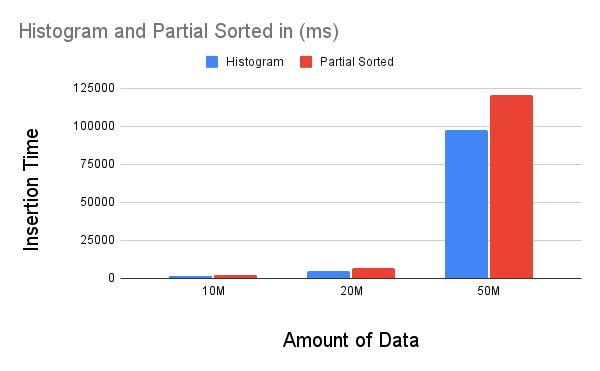
\includegraphics[width=100mm,scale=1]{Figures/InsertionScalability.png}
    \caption{
     Results of Insertion Operation on different test sizes (Gaussian Distribution)
    }
    \label{fig:InsertionScalability}
\end{figure}
Insertion time shows a similar trend to query performance (Figure \ref{fig:InsertionScalability}), where the histogram outperforms the partially sorted approach as the data size increases. When the data size is small, the partially sorted approach tends to outperform the histogram because it delays new node creation, while the histogram creates a new node only when there is a conflict. However, when the amount of data increases, and more partially sorted keys are inserted into each node, the performance of the partially sorted approach worsens as it has to perform recursive rebuilding. This slows down the insertion performance compared to the histogram since the recursive rebuilding cost is $O(\frac{N}{2})$, where $N$ is the number of keys in the node.

When it comes to query and insertion performance in real-world datasets, we have seen that the histogram approach may not be as effective as it is in the Gaussian distribution. However, the general trend of histogram outperforming partially sorted is still observed. This is because, in histogram, we only need to traverse down the tree depth to locate the keys, whereas in partially sorted, we need to perform local search similar to \acrshort{alex}\cite{ALEX}. As the amount of data increases, the number of partially sorted keys also increases, which in turn increases the depth of the tree. Therefore, we observe a linear increase in partially sorted performance with increasing data size. However, histogram can still create new nodes and increase the tree depth without the need for local search, making it more scalable than the partially sorted approach.

Furthermore, the trend in insertion performance is also similar to that of query performance. When the amount of data is small, partially sorted tends to outperform the histogram as it delays the creation of new nodes. However, as more data is inserted into the tree, the number of partially sorted keys in each node increases, which triggers recursive rebuilding that can slow down the insertion performance. In contrast, the histogram approach still outperforms partially sorted because it only needs to traverse down the tree depth and create new nodes when there is a conflict, without the need for local search. This makes the insertion operation faster in histogram than in partially sorted.

In summary, the histogram approach is more scalable than the partially sorted approach for both query and insertion operations, especially when dealing with large amounts of data, as histogram does not require any extra searches after traversing down the tree compared to partially sorted keys.
